\documentclass{beamer}

\usepackage{beamerthemesplit}
\usepackage[utf8]{inputenc}
\usepackage[polish]{babel}
\usepackage[T1]{fontenc}
\usetheme{Warsaw}
\setbeamertemplate{navigation symbols}{}

\title[Konwersja na Active~Record\hspace{10em}\insertframenumber/\inserttotalframenumber]{Konwersja bazy danych na format zgodny z Active~Record}
\author{Igor Rzegocki}
\date{\today}
\institute{Akademia Górniczo-Hutnicza}

\begin{document}

\begin{frame}
  \titlepage
\end{frame}

\begin{frame}
  \frametitle{Plan Prezentacji}
  \tableofcontents
\end{frame}

\section{Bardzo Szybkie Omówienie Active~Record}
\subsection{Co To Jest u Licha?}
\begin{frame}
  \frametitle{Co To Jest u Licha?}
  \begin{itemize}
  \uncover<1->{\item Active~Record to ORM}
    \begin{itemize}
    \uncover<2->{\item a ściślej jedna z jego implementacji}
    \uncover<3->{\item a co to jest ORM?}
    \end{itemize}
  \uncover<4->{\item Implementacje Active~Record są tworzone z myślą o klientach Media~Markt...}
    \begin{itemize}
    \uncover<5->{\item Microsoftu...}
    \uncover<6->{\item Amerykanach...}
    \uncover<7->{\item ...i wszystkich innych, którzy z jakiegoś powodu nie potrafią się nauczyć SQL}
    \end{itemize}
  \uncover<8->{\item Dlaczego więc się go wdraża?}
    \begin{itemize}
      \uncover<9->{\item ...przecież nie wszyscy programiści kupują w Media~Markt}
    \end{itemize}
  \end{itemize}
\end{frame}
\subsection{Jak To Działa?}
\begin{frame}[fragile]
  \frametitle{Jak To Działa?}
  \begin{itemize}
    \item Jak to działa? Bardzo prosto!
  \end{itemize}
  \begin{block}{Przykładowa Tabelka}
    \scriptsize
    \begin{verbatim}
 +---------------+-------------+------+-----+---------+----------------+
 | Field         | Type        | Null | Key | Default | Extra          |
 +---------------+-------------+------+-----+---------+----------------+
 | id            | int(11)     | NO   | PRI | NULL    | auto_increment | 
 | login         | varchar(20) | NO   |     | NULL    |                | 
 | password      | varchar(40) | NO   |     | NULL    |                |
 +---------------+-------------+------+-----+---------+----------------+
    \end{verbatim}
    \normalsize
  \end{block}
  \pause
  Pytanie bonusowe: Dlaczego `password` jest varchar(40)?
\end{frame}
\begin{frame}
  \frametitle{Jak To Działa? - Zapis}
  \uncover<1->{
    \begin{block}{Zapis do bazy}
      user = User.new\newline
      user.login = 'ajgon'\newline
      user.password = Digest::SHA1.hexdigest('wyindywidualizowany')\newline
      user.save!
    \end{block}
  }
  \uncover<2->{
    \begin{block}{Zapis do bazy - Kod SQL}
      INSERT INTO users (login, password) VALUES ('ajgon', '4aa7ed795f2de0ef0bd961d2c4282a2a4d0adafa')
    \end{block}
  }
\end{frame}
\begin{frame}
  \frametitle{Jak To Działa? - Odczyt}
  \uncover<1->{
    \begin{block}{Odczyt z bazy}
      User.find(:all) \# => zwraca tablicę\newline
      User.find(:first) \# => zwraca obiekt\newline
      User.find(42).login \# => zwraca string 'ajgon'\newline
    \end{block}
  }
  \uncover<2->{
    \begin{block}{Odczyt z bazy - Kod SQL}
      SELECT * FROM users\newline
      SELECT * FROM users LIMIT 1\newline
      SELECT * FROM users WHERE id = 42\newline
    \end{block}
  }
\end{frame}
\subsection{Problemy}
\begin{frame}
  \frametitle{Problemy w Active~Record}
  \begin{itemize}
  \uncover<1->{\item Jeśli kolumna w bazie nazywa się inaczej niż `id` skąd model ma wiedzieć po czym szukać?}
  \uncover<2->{\item W każdym modelu trzeba osobno deklarować nazwę tabeli, kodowanie etc.}
  \uncover<3->{\item Co z kluczami? Zrobienie JOINa wiąże się ze wstrzykiwaniem SQLa}
  \uncover<4->{\item I mnóstwo innych, nie do przeskoczenia dla klienta Media~Markt :-)}
  \end{itemize}
\end{frame}
\begin{frame}
  \frametitle{Problemy w Active~Record - Rozwiązanie}
  \begin{itemize}
    \uncover<1->{\item Rozwiązanie? Convention~over~Configuration}
    \begin{itemize}
      \uncover<2->{\item Niezależnie od tego jak bardzo informatycy kochają trzyliterowe akronimy, tej nazwy się NIE skraca}
      \uncover<3->{\item Convention~over~Configuration nie należy do modelu Active~Record i jest rozdawany oddzielnie}
      \uncover<4->{\item Przed użyciem zapoznaj się z dokumentacją lub skonsultuj się z informatykiem lub programistą}
    \end{itemize}
    \uncover<5->{\item Znormalizowane nazwy - kolumna indeksująca MUSI się nazywać `id` i jest obowiązkowa}
    \uncover<6->{\item Model jest liczbą pojedyńczą a nazwa tabeli liczbą mnogą}
    \begin{itemize}
      \uncover<7->{\item Istnieje cała klasa Pluralize w Ruby~on~Rails, która odpowiada za wszystkie wyjątki}
      \uncover<8->{\item Oznacza to także, że wymusza to nazywanie tabel w języku angielskim - bardzo dobry nawyk!}
    \end{itemize}
    \uncover<9->{\item Nazwy kluczy są również znormalizowane - liczba\_pojedyńcza\_id}
  \end{itemize}
\end{frame}
\section{Konwersja Bazy Danych}
\subsection{Problemy}
\begin{frame}
  \frametitle{Co Należało Skonwertować?}
  \begin{itemize}
    \uncover<1->{\item Dana jest baza danych strony http://eit.agh.edu.pl/}
    \begin{itemize}
      \uncover<2->{\item A dokładniej jej struktura}
    \end{itemize}
    \uncover<3->{\item Pierwsze wrażenie?}
  \end{itemize}
  \begin{center}
    \uncover<4->{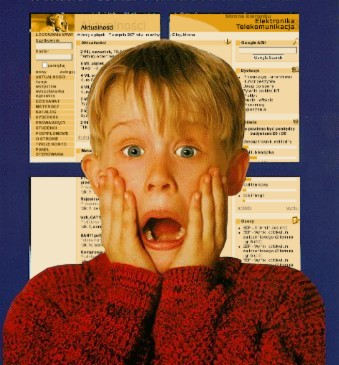
\includegraphics[scale=0.4]{kevin.jpg}}
  \end{center}
\end{frame}
\begin{frame}
  \frametitle{Błędy w Starej Bazie Danych}
  \setbeamercovered{transparent}
  \begin{itemize}
    \uncover<1->{\item Brak jakiejkolwiek logiki w nazywaniu kolumn}
    \uncover<2->{\item Niektóre kolumny są słowami polskimi, niektóre angielskimi, a niektóre nic nie mówiącymi skrótami}
    \uncover<3->{\item Brak kluczy obcych}
    \uncover<4->{\item Baza w żaden sposób nie pilnuje danych}
    \uncover<5->{\item Całkowicie zepsute kodowanie znaków}
    \uncover<6->{\item I wiele innych, pomniejszych...}
  \end{itemize}
\end{frame}
\subsection{Koncepcje Konwertera}
\begin{frame}
  \frametitle{Koncepcje Konwertera}
  \begin{itemize}
    \uncover<1->{\item Pierwsza koncepcja - kod konwertujący}
    \begin{itemize}
      \uncover<2->{\item Nigdy, PRZENIGDY tego nie róbcie!}
    \end{itemize}
    \uncover<3->{\item Druga koncepcja - plik konfiguracyjny}
    \begin{itemize}
      \uncover<4->{\item Bardzo dobre rozwiązanie}
      \uncover<5->{\item Plik konfiguracyjny - YAML}
    \end{itemize}
  \end{itemize}
\end{frame}
\subsection{Uwzględnione Funkcjonalności}
\begin{frame}
  \frametitle{Uwzględnione Funkcjonalności}
  \setbeamercovered{transparent}
  \begin{itemize}
    \uncover<1->{\item Zmiana nazw kolumn}
    \uncover<2->{\item Usuwanie niepotrzebnych kolumn}
    \uncover<3->{\item Zachowanie relacji i pogodzenie ich z kluczami}
    \begin{itemize}
      \uncover<3->{\item Czasami mapowanie nie było po id (sic!)}
    \end{itemize}
    \uncover<4->{\item Nakładanie funkcji SQLowych na dane}
    \uncover<5->{\item Poprawianie starych tabel przed i po konwersji}
    \uncover<6->{\item Konwertowanie tylko wierszy spełniających określony warunek}
  \end{itemize}
\end{frame}
\section{Krótka Informacja o Mojej Pracy Magisterskiej}
\subsection{Tytuł i Autor Pracy}
\begin{frame}
  \frametitle{Tytuł i Autor Pracy}
  \title{Migracja serwisu WWW z techniki PHP na Ruby~on~Rails}
  \author{Igor Rzegocki}
  \date{}
  \institute{}
  \titlepage
\end{frame}
\subsection{Opiekun Pracy}
\begin{frame}
  \frametitle{Opiekun Pracy}
  \begin{center}
    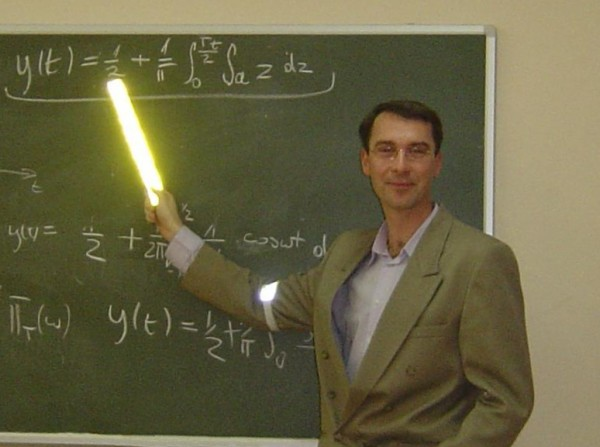
\includegraphics[scale=0.35]{juszkiew.jpg}
  \end{center}
  \begin{center}
    dr inż. Krzysztof Juszkiewicz
  \end{center}
\end{frame}
\subsection{Cel Pracy}
\begin{frame}
  \frametitle{Cel Pracy}
  \begin{columns}
    \column{0.5\textwidth}
    \uncover<1->{
    \begin{center}
      Migracja z takiego serwisu...
      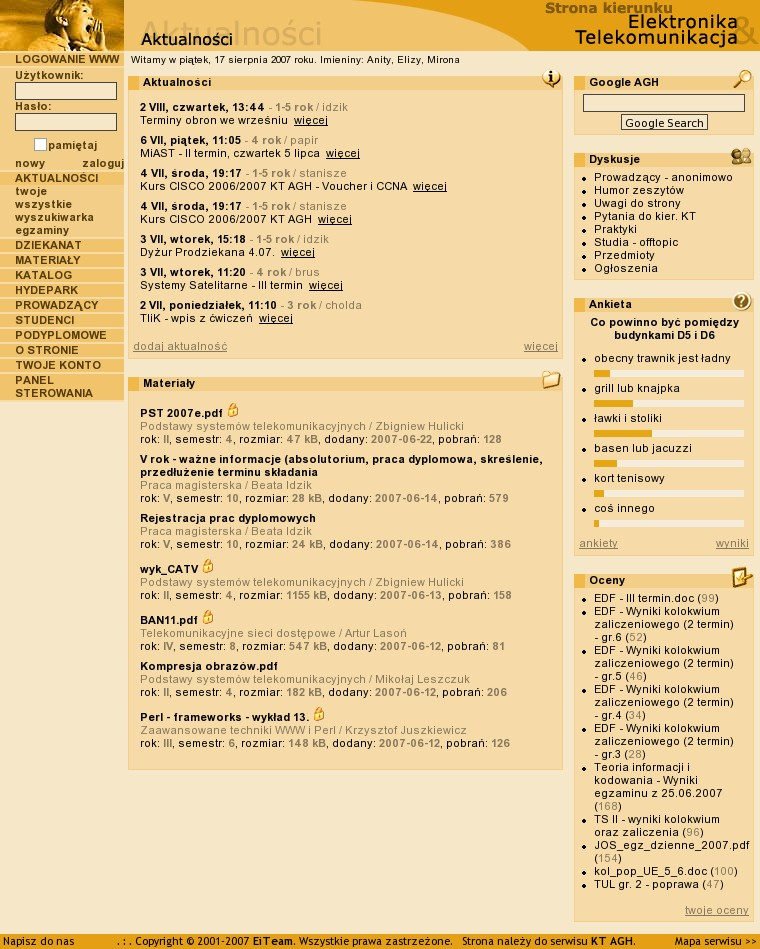
\includegraphics[scale=0.2]{eit.jpg}
    \end{center}
    }
    \column{0.5\textwidth}
    \uncover<2->{
    \begin{center}
      ...na taki :-)
      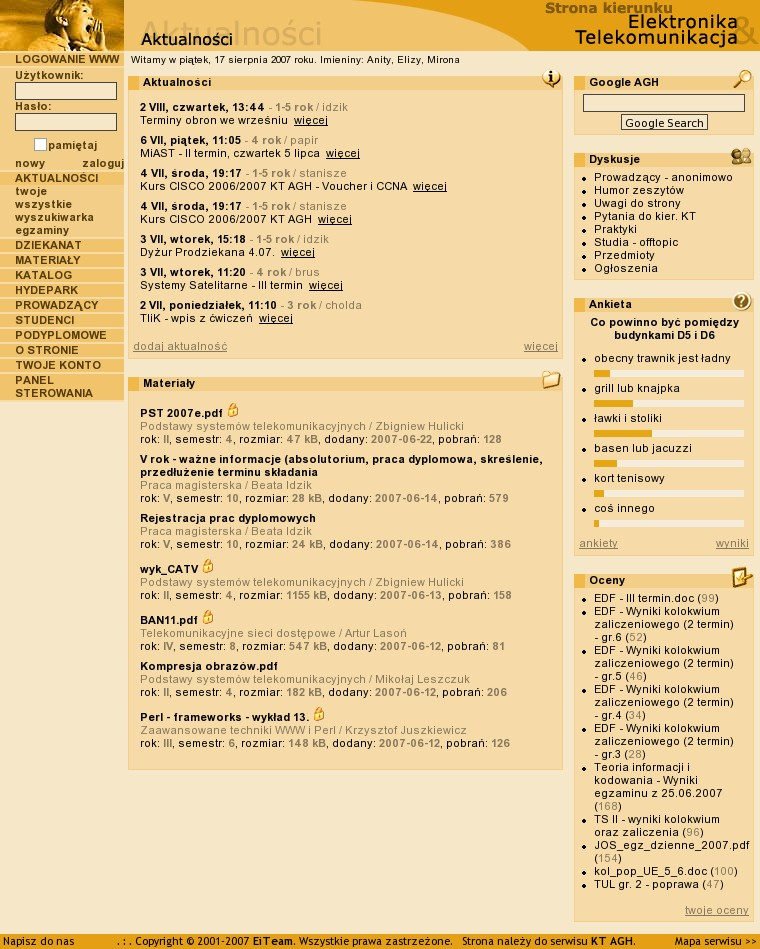
\includegraphics[scale=0.2]{eit.jpg}
    \end{center}
    }
  \end{columns}
\end{frame}
\section{}
\begin{frame}
  \begin{center}
  \huge
  \uncover<1->{Dziękuję za uwagę!}\newline
  \normalsize
  \uncover<2->{...and thanks for all the fish :-)}
  \end{center}
\end{frame}
\end{document}

